\documentclass{article}

\usepackage{amsmath}
\usepackage{amsfonts}
\usepackage{amssymb}
\usepackage{graphicx}
\usepackage{float}
\usepackage{hyperref}
\usepackage{subfig}
\usepackage{url}
\usepackage{minted}
\usepackage[margin=0.75in]{geometry}
\graphicspath{{./assets/}}

\begin{document}

\section{Introduction}

    One time when I was binging YouTube, I stumbled upon a video by Grant Sanderson
    of 3Blue1Brown on Fourier series which featured many visualizations, prime of
    whose were drawings on a complex plain which were generated using Fourier
    series. Having done some reading on Fourier series as well as Fourier transform, 
    I decided that it would be a great idea to actually understand those concepts.
    Since for me the ultimate way of learning is solving problems and since I feel
    best at expressing ideas in code, I decided to set myself a challenge of 
    programming a program that will redraw my sketches with Fourier series.


\section{What is Fourier series?}

    The purpose of Fourier series is to approximate any periodic function with
    a sum of sines and cosines. The formula is given by~\eqref{eq:fs_rbase}
    \begin{equation} \label{eq:fs_rbase}
        S_\infty(t) = a_0 + \sum_{n=1}^{\infty}a_ncos\frac{2\pi nt}{P} + b_n%
            sin\frac{2\pi nt}{P}
    \end{equation}
    From the formula we can observe two things, each sine and cosine in the sum
    has a weight assigned to it ($a_n$ and $b_n$) and that $n$ determines the 
    frequency of the sinusoids. We can demistify the idea behind Fourier series
    by deriving formulas for all coefficients.

\subsection{Deriving $a_0$}
    
    First coefficient we will find is $a_0$, which is the only coefficient that 
    stands on its own. It is added before the actual series in order to compensate
    for the original function not oscillating around $x$ axis on the plot. It 
    basically is a vertical translation. We can see it if we add any constant
    to $sin(x)$~\ref{fig:sine_translation}.
    \begin{figure}[H]
        \caption{red - $sin(x)$, blue - $3 + sin(x)$}
        \centering
        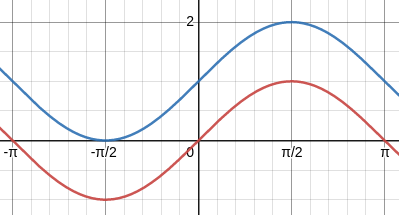
\includegraphics[width=0.5\linewidth]{translated_vanilla_sinewave}
        \label{fig:sine_translation}
    \end{figure}
    Now the problem to solve is what it the axis around which our sum of sines
    and cosines is to oscillate against. The solution to this problem is the average
    value of the original function over one period. The formula given for finding
    $a_0$ goes as follows~\eqref{eq:a0_formula}
    \begin{equation}\label{eq:a0_formula}
        a_0 = \frac{1}{P}\int_{\frac{P}{2}}^{\frac{-P}{2}}f(t)dt
    \end{equation}
    Now, how does an integral grant us mean value of a function? Well, definite
    integral gives us the area under the graph of function $f(t)$ from 
    $-\frac{1}{P}$ to $\frac{1}{P}$. If we have an area, we can express it with 
    any figure that has this area, since we want an offset from the $x$ axis, 
    we can draw a rectangle whose base has length of $P$. Since we want to find
    out what the height of that rectangle is, we need to divide its area by its
    width, which is exactly what we are doing when dividing the integral by $P$.

\subsection{Finding $a_n$ and $b_n$}

    Weights $a_n$ and $b_n$ allow for the series to converge to desired function, 
    which is quite obvious from the fact that the series is infinite, which means
    that the values on their own would shoot up to infinity. Now, how are we to 
    find those weights to force the sinusoids to compliance? We can start with 
    equating some function $f(t)$ to a Fourier series~\eqref{eq:eq_fs_f(t)}
    \begin{equation} \label{eq:eq_fs_f(t)}
        f(t) = a_0 + \sum_{n=1}^{\infty}a_ncos\frac{2\pi nt}{P} + b_n%
            sin\frac{2\pi nt}{P}
    \end{equation}
    In order to find the coefficients, we can exploit the properties of definite
    integrals of sine and cosine. To do that, we will need to expand the whole 
    expression by either $cos\frac{2\pi nt}{P}$ when looking for $a_n$, or by 
    $sin\frac{2\pi nt}{P}$ if we are looking for $b_n$. Now we will go through 
    the whole process by looking for $a_n$. 


    The expanded equation we will use to find $a_n$ looks like this~\eqref{eq:fs_exp_cos}.
    \begin{equation}\label{eq:fs_exp_cos}
    \begin{split}
        \int_{-\frac{P}{2}}^{\frac{P}{2}}f(t)cos\frac{2\pi nt}{P}dt 
        = \int_{-\frac{P}{2}}^{\frac{P}{2}}a_0cos\frac{2\pi nt}{P}dt 
        & +\int_{-\frac{P}{2}}^{\frac{P}{2}}a_1cos\frac{2\pi t}{P}cos\frac{2\pi nt}{P}dt +
        \int_{-\frac{P}{2}}^{\frac{P}{2}}b_1sin\frac{2\pi t}{P}cos\frac{2\pi nt}{P}dt \\
        & + \int_{-\frac{P}{2}}^{\frac{P}{2}}a_2cos\frac{4\pi t}{P}cos\frac{2\pi nt}{P}dt +
        \int_{-\frac{P}{2}}^{\frac{P}{2}}b_2sin\frac{4\pi t}{P}cos\frac{2\pi nt}{P}dt \\
        & \vdots \\
        & + \int_{-\frac{P}{2}}^{\frac{P}{2}}a_ncos^2(\frac{2\pi nt}{P})dt +
        \int_{-\frac{P}{2}}^{\frac{P}{2}}b_nsin\frac{2\pi nt}{P}cos\frac{2\pi nt}{P}dt 
    \end{split}
    \end{equation}
    From this rather long expansion we can distill and solve for five cases appearing
    on the right side of the equation:
    \begin{enumerate}
        \item \begin{equation*}
                \int_{-\frac{P}{2}}^{\frac{P}{2}}a_0cos\frac{2\pi nt}{P}dt
                = a_0 \cdot \left[\frac{P}{2\pi nt}sin\frac{2\pi nt}{P}\right]_{-\frac{P}{2}}^{\frac{P}{2}}
                = a_0 \cdot \frac{P}{2\pi nt}(sin(\pi n) - sin(-\pi n)) = 0
              \end{equation*}
        \item let $m \in Z \land m \neq n$
            \begin{equation*}
            \begin{split}
                \int_{-\frac{P}{2}}^{\frac{P}{2}}a_mcos\frac{2\pi mt}{P}cos\frac{2\pi nt}{P}dt 
                & = a_m \cdot \int_{-\frac{P}{2}}^{\frac{P}{2}}\frac{1}{2}\left(cos\frac{(m-n)2 \pi t}{P} + 
                cos\frac{(m+n)2 \pi t}{P}\right)dt \\
                & = a_m \cdot \left[\frac{P}{4\pi(m-n)}sin\frac{(m-n)2 \pi t}{P}
                + \frac{P}{4\pi(m+n)}sin\frac{(m+n)2 \pi t}{P}\right]_{-\frac{P}{2}}^{\frac{P}{2}} \\
                & = a_m \cdot (\frac{P}{4\pi(m-n)}sin((m-n)\pi) + \frac{P}{4\pi(m+n)}sin(-(m+n)\pi) = 0
            \end{split}
            \end{equation*}
        \item let $m \in Z$
            \begin{equation*}
            \begin{split}
                \int_{-\frac{P}{2}}^{\frac{P}{2}}b_msin\frac{2\pi mt}{P}cos\frac{2\pi nt}{P}dt 
                & = b_m \cdot \int_{-\frac{P}{2}}^{\frac{P}{2}}\frac{1}{2}\left(sin\frac{(m+n)2 \pi t}{P} + 
                sin\frac{(m+n)2 \pi t}{P}\right)dt \\
                & = b_m \cdot \left[\frac{-P}{4\pi(m+n)}cos\frac{(m+n)2 \pi t}{P}
                + \frac{-P}{4\pi(m+n)}cos\frac{(m+n)2 \pi t}{P}\right]_{-\frac{P}{2}}^{\frac{P}{2}} \\
                & = b_m \cdot (\frac{-P}{4\pi(m-n)}cos((m-n)\pi) + \frac{-P}{4\pi(n+m)}cos(-(m+n)\pi) = 0
            \end{split}
            \end{equation*}
        \item 
            \begin{equation*}
            \begin{split}
                \int_{-\frac{P}{2}}^{\frac{P}{2}}cos^2(\frac{2\pi nt}{P})dt
                & = \frac{1}{2}\int_{-\frac{P}{2}}^{\frac{P}{2}}1 + cos\frac{4\pi nt}{P}dt 
                = \frac{1}{2} \cdot \left[t + \frac{P}{4\pi nt}sin\frac{4\pi nt}{P}
                \right]_{-\frac{P}{2}}^{\frac{P}{2}} \\
                & = \frac{1}{2} \cdot \left(\frac{P}{2} + \frac{1}{2\pi n}sin(2\pi n)
                + \frac{P}{2} + \frac{1}{2\pi n}sin(-2\pi n)\right) = \frac{2}{P}
            \end{split}
            \end{equation*}
    \end{enumerate}

    We can see that the only term after expansion and integration that does not 
    amount to zero is $\int_{-\frac{P}{2}}^{\frac{P}{2}}cos^2(\frac{2\pi nt}{P})dt$,
    which means that our equation will simplify to the following form~\eqref{eq:fs_simp_cos}
    \begin{equation}\label{eq:fs_simp_cos}
        \int_{-\frac{P}{2}}^{\frac{P}{2}}f(t)cos\frac{2\pi nt}{P}dt = a_n\frac{P}{2}
    \end{equation}
    So in order to find $a_n$, we will get the following\eqref{eq:a_n}
    \begin{equation}\label{eq:a_n}
        a_n = \frac{2}{P}\int_{-\frac{P}{2}}^{\frac{P}{2}}f(t)cos\frac{2\pi nt}{P}dt
    \end{equation}
    Formula for $b_n$ is very similar~\eqref{eq:b_n} and stems from the same logic as one of 
    $a_n$, see Appendix A for calculations.
    \begin{equation}\label{eq:b_n}
        b_n = \frac{2}{P}\int_{-\frac{P}{2}}^{\frac{P}{2}}f(t)sin\frac{2\pi nt}{P}dt
    \end{equation}

\subsection{Approximating a step function}
    
    Before diving straight to other concepts and the drawings, let us 
    take a second and manually approximate a step function defined in ~\eqref{eq:step}
    and plotted in Figure~\ref{fig:step_func}

    \begin{equation}\label{eq:step}
    \begin{split}
         &f(t) = 
        \begin{cases} 
            & -2 \text{ if } -\pi \leq t < 0 \\
            & 2 \text{ if }  0 \leq t \leq \pi
        \end{cases} \\
        & f(t) = f(t + 2\pi) 
    \end{split}
    \end{equation}

    \begin{figure}[H]
        \caption{Step function f(t)}
        \centering
        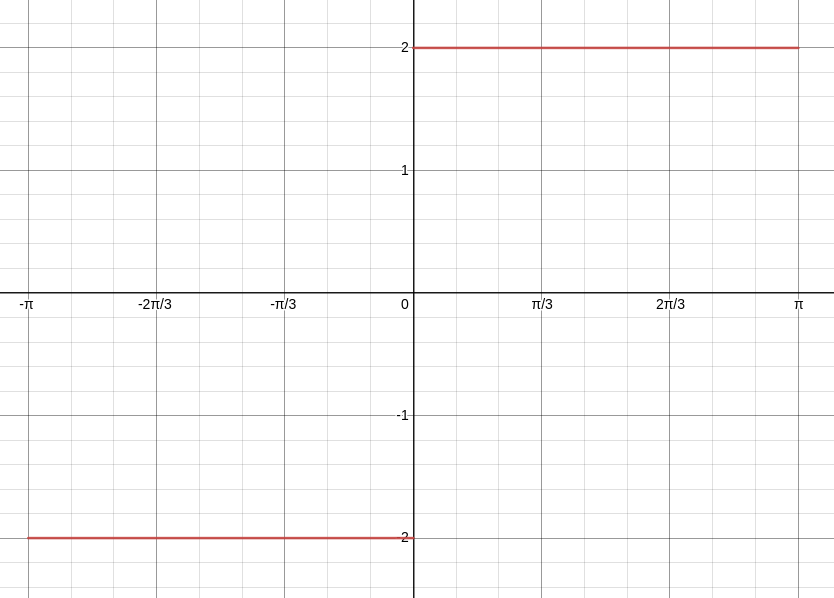
\includegraphics[width=0.5\linewidth]{step_func}
        \label{fig:step_func}
    \end{figure} 


    If we look on the graph, we can already establish that the definite integral
    of the function over the whole period is zero, hence $a_0 = 0$. \\


    Other thing we want to observe is that the function $f(t)$ is odd, meaning
    that \textbf{$f(t) = -f(-t)$} and the function that is odd in our series is
    the sine, we know that all coefficients $a_n$ will be zero because otherwise
    they would distort our approximation.
    \begin{equation}
    \begin{split}
        b_n & = \frac{2}{\pi}\int_{-\pi}^{\pi}f(t)sin(nt)dt 
        = \frac{2}{\pi} \cdot \left[f(t)\cdot t \cdot \frac{1}{-nt}cos(nt)\right]_{-\pi}^{\pi} \\
        & = \frac{2}{\pi} \cdot \left[\frac{2}{n}\left(cos(n\pi) + cos(n\pi)
        - (-cos(-(n\pi) + cos(-n\pi) \right)\right] \\
        & = \frac{4}{n\pi}\left(2cos(n\pi) + 2cos(-n\pi)\right) = 
        \begin{cases} 
            & \frac{8}{n\pi} \text{ if n is odd} \\
            & 0 \text{ if n is even}
        \end{cases} 
    \end{split}
    \end{equation}
    
    The series for our step function looks like this~\eqref{eq:step_fs}
    \begin{equation}\label{eq:step_fs}
        S_\infty(t) = \sum_{n=1}^{\infty}\frac{8}{(2n-1)\pi}sin((2n - 1)t)
    \end{equation}

    Now we can make a few plots of the series with increasing number of terms
    and see it converge to $f(t)$, Figure~\ref{step_fs_plots}
    \begin{figure}[H]
    \caption{}
    \begin{tabular}{cc}
    \subfloat[n = 0]{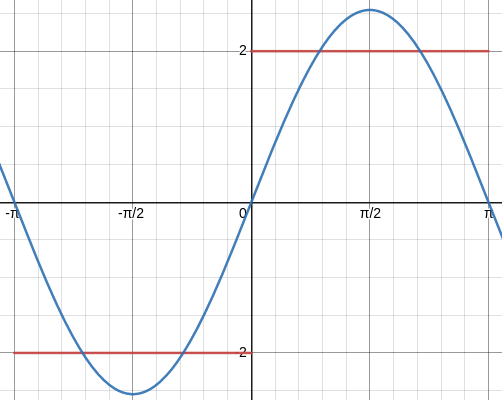
\includegraphics[width=0.4\linewidth]{step_approx_1}} &
    \subfloat[n = 2]{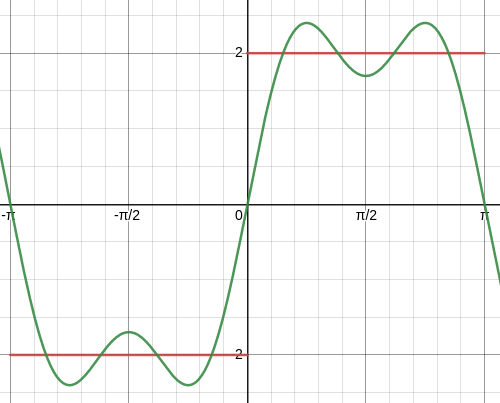
\includegraphics[width=0.4\linewidth]{step_approx_2}}\\
    \subfloat[n = 5]{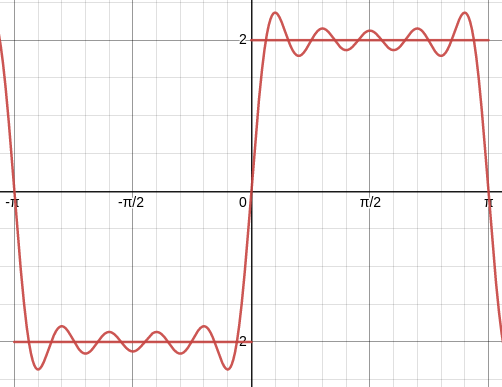
\includegraphics[width=0.4\linewidth]{step_approx_3}} &
    \subfloat[n = 7]{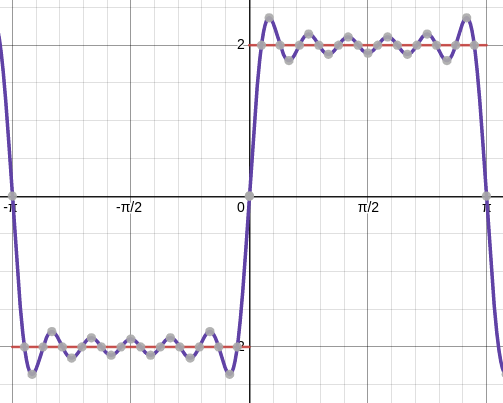
\includegraphics[width=0.4\linewidth]{step_approx_4}}
    \end{tabular}
    \label{step_fs_plots}
    \end{figure}

    We now know what the pure form of Fourier series is, but now we need to use it to
    draw images, so from now on, we will keep on walking through all the concepts, 
    but in the context of the program itself.


\section{Overview of the program} 

    The program has three main stages:
    \begin{enumerate}
        \item taking input from the user and mapping it onto complex plane
        \item processing the input using discrete Fourier transform (DFT)
        \item redrawing the sketch using complex form of Fourier series
    \end{enumerate}

    In this short list we have two completely new concepts and one slightly 
    mutated, so let us now go through each component in their applied form.

\subsection{Complex numbers}

    A drawing in case of the program is a set of $x$ and $y$ coordinates, however,
    for all calculations we need something called complex numbers. Akin to points
    that are desrcibed in terms of coordinates, complex numbers are described in
    two dimensions. One of them everyone knows really well, because this is the 
    the real component, which, as the name suggests, consists of real numbers.
    The component that allows us to move vertically does not belong on the real 
    number line because this number is $\sqrt{-1}$, usually denoted as $i$. So
    any complex number can be denoted as following: $a + bi$ and can be depicted
    like in figure~\ref{fig:complex_number}
    \footnote{Graphic taken from \url{https://en.wikipedia.org/wiki/Complex_number}}
    \begin{figure}[H]
        \caption{}
        \centering
        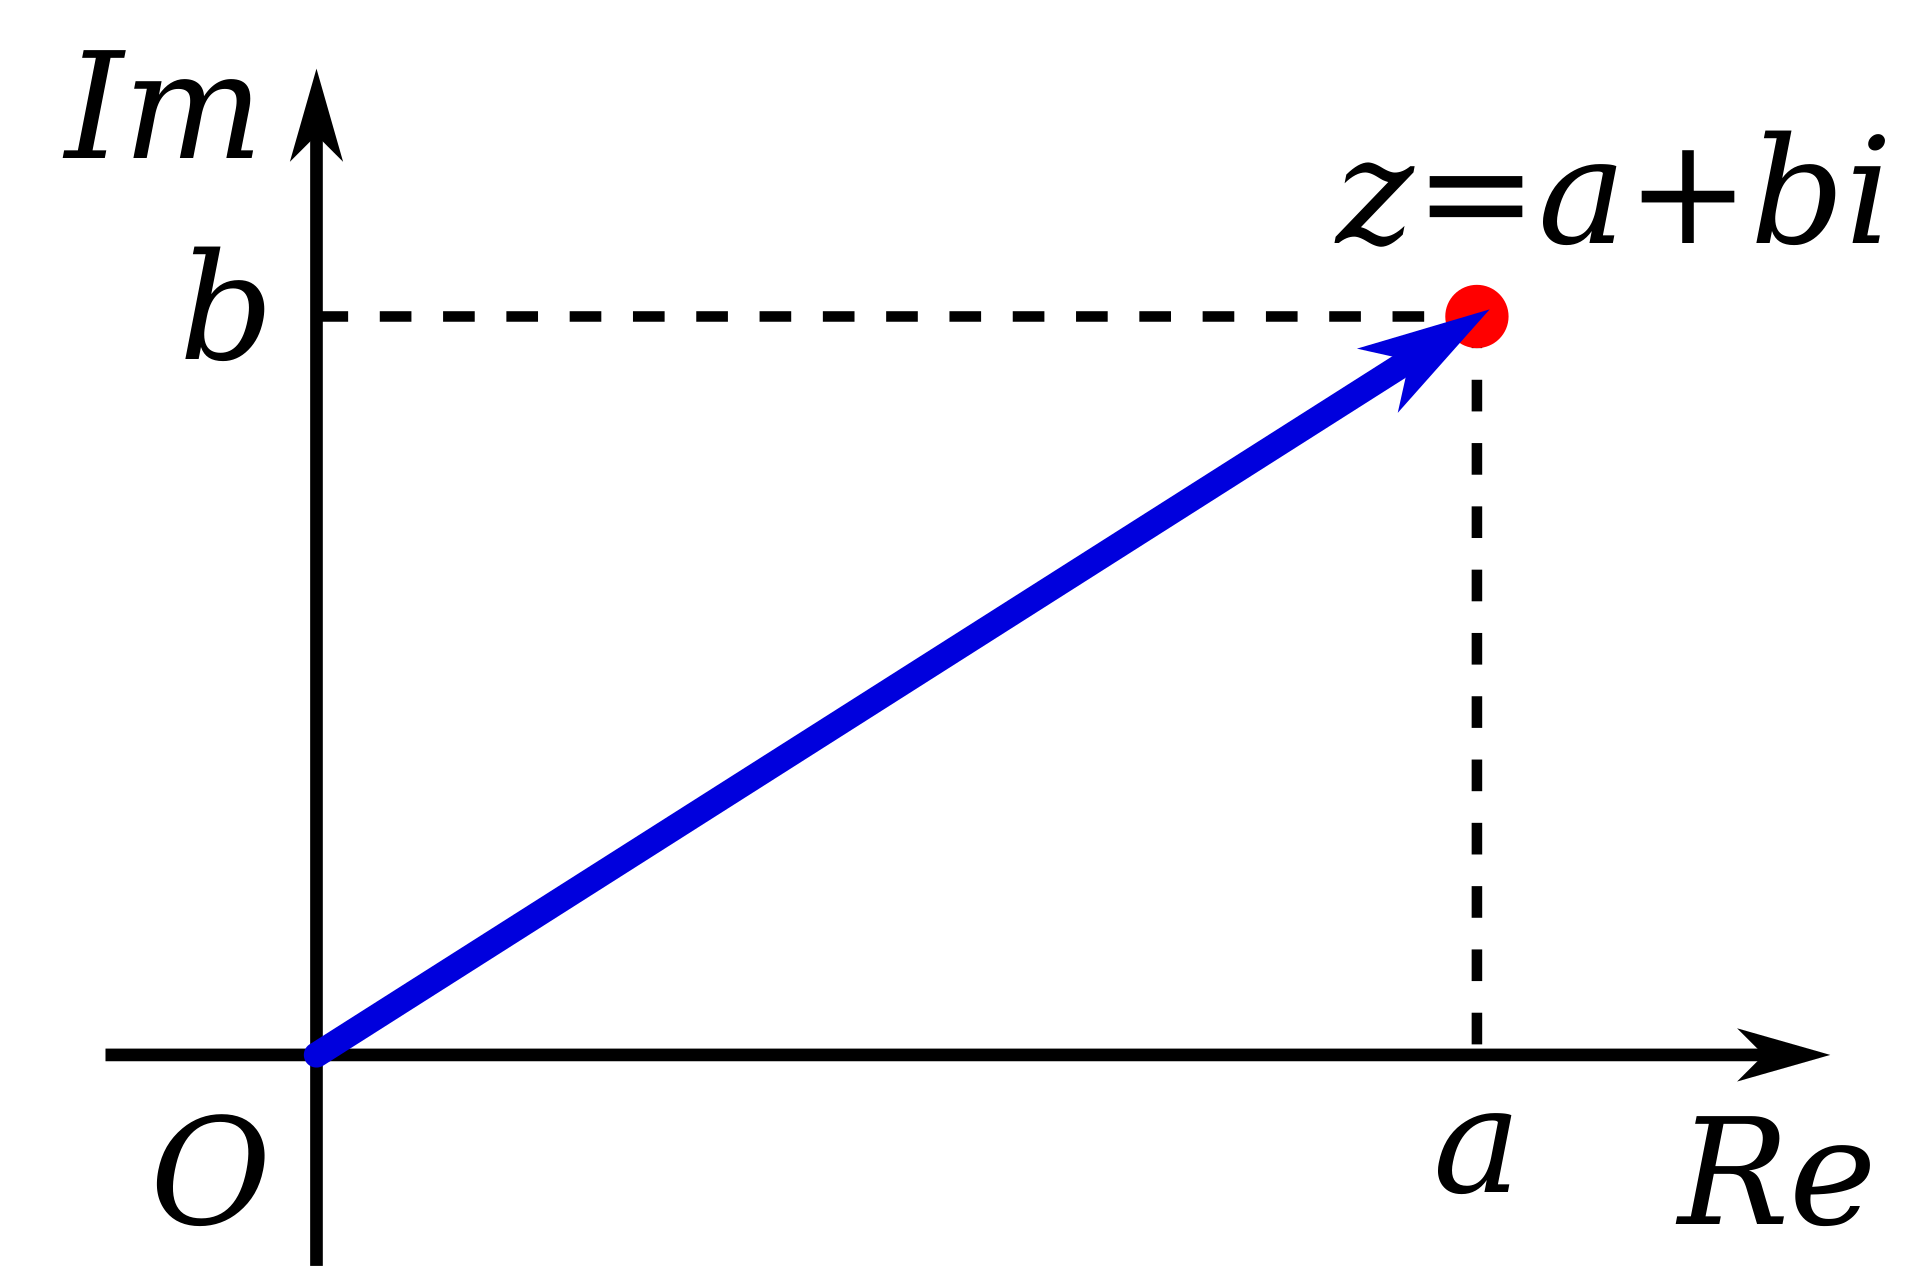
\includegraphics[width=0.3\linewidth]{imaginary_number}
        \label{fig:complex_number}
    \end{figure}
    The arithmetics with complex numbers look exactly the same like in case of 
    any other numbers.
    
    It is already apparent why we would use a set complex numbers when trying 
    to draw instead, for example a function like we did in previous section. 
    It gives us two dimensions of freedom which is excactly what we need since
    our sketches will be two-dimensional.


\subsection{Discrete Fourier transform (DFT)}

    Next step in the program is to find the coefficients for the Fourier series
    to work with. However, the process will be a bit different since
    we are working with a set of complex numbers rather than a real-valued function.
    This is where DFT, or discrete Fouirer transform comes into play. Remember
    how the coefficients $a_n$ and $b_n$ described the amplitude of sinusoids with
    frequency of $n$? What Fourier transform does is finding the amplitude of 
    signals with given frequency. The formula for DFT is as follows~\eqref{eq:dft_vanilla}.
    \begin{equation}\label{eq:dft_vanilla}
        X_k = \sum_{n=0}^{N-1}x_n \cdot \left[cos\left(\frac{2\pi}{N}kn\right) - 
        isin\left(\frac{2\pi}{N}kn\right)\right]
    \end{equation}
    Now let us walk through what each variable means:
    \begin{itemize}
        \item $X_k$ - output complex number of DFT
        \item $N$ - size of input set
        \item $k$ - frequency
        \item $x_n$ - $n^{th}$ complex number in the input set
    \end{itemize}
    
    The first thing to go through is why we are multiplying our input complex 
    number by a complex sum?

\subsubsection{Expressing a point on a unit circle using complex numbers}

    Let us take a right triangle with hypotenuse of length $1$~\ref{fig:right_triangle}
    and angle $\theta$ between that hypotenuse ($c$) and the base $b$ of triangle.
    \begin{figure}[H]
        \caption{}
        \centering
        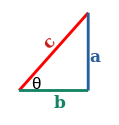
\includegraphics[width=0.2\linewidth]{right_triangle}
        \label{fig:right_triangle}
    \end{figure}
    If we wanted to find the length of the base ($b$), it would be equal
    to the $cos\theta$ since the hypotenuse has the length $1$. Similarly, if we
    wanted to find the height of the triangle ($a$), it would be the $sin\theta$.

    Now we can inscribe such right triangle into a unit circle on a complex plane
    where the hypotenuse of the triangle would simultaneusly be the radius of 
    the triangle~\ref{fig:inscribed_triangle} with some angle $\theta$ between
    radius and the horizontal axis.
    \begin{figure}[H]
        \caption{}
        \centering
        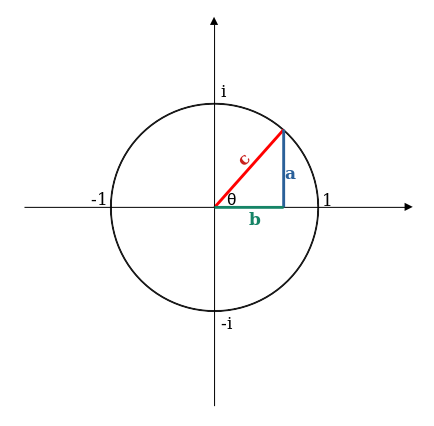
\includegraphics[width=0.4\linewidth]{inscribed_triangle}
        \label{fig:inscribed_triangle}
    \end{figure}
    We can find the coordinate of the point where the radius touches the circumference
    using the inscribed triangle, so $cos\theta$ would be the horizontal coordinate
    and $i \cdot sin\theta$ would be the vertical component since we are on complex
    plane. So the whole position can be described as $cos\theta + isin\theta$.


\subsubsection{The crux of DFT matter}

    Now, having the basis, we can go through the DFT inductively. Let us find 
    Fourier transform for $cos(2t)$. We already know that the expression 
    $cos\left(\frac{2\pi}{N}kn\right) - isin\left(\frac{2\pi}{N}kn\right)$ describes
    unit circle on a complex plane. What we are doing with DFT mapping our input
    set around this unit circle - Figure~\ref{fig:cos_wrapped}. In plot $(b)$ we
    can see the heart of Fouerier transform. Since we are summing all numbers in 
    the set, and, as we can see, the plot is symmetrical, so all the values will 
    cancel out, leaving us with 0.
    \begin{figure}[H]
      \caption{}\label{fig:cos_wrapped}
      \centering
        \subfloat[$cos(2t)$]{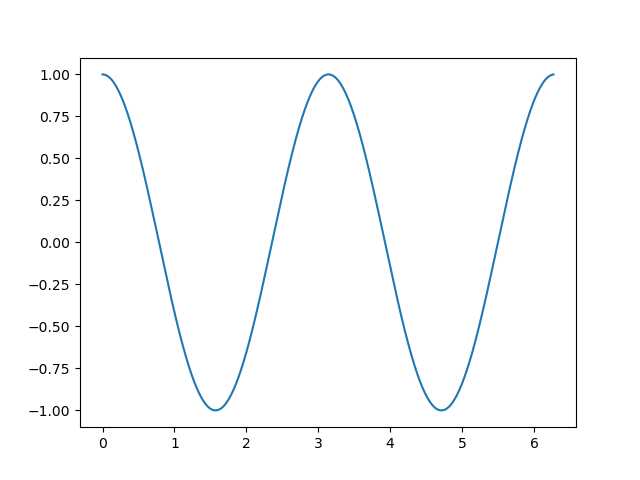
\includegraphics[width=0.4\textwidth]{cos_vanilla}}
      \hfill
        \subfloat[$cos(2t)$ - wrapped]{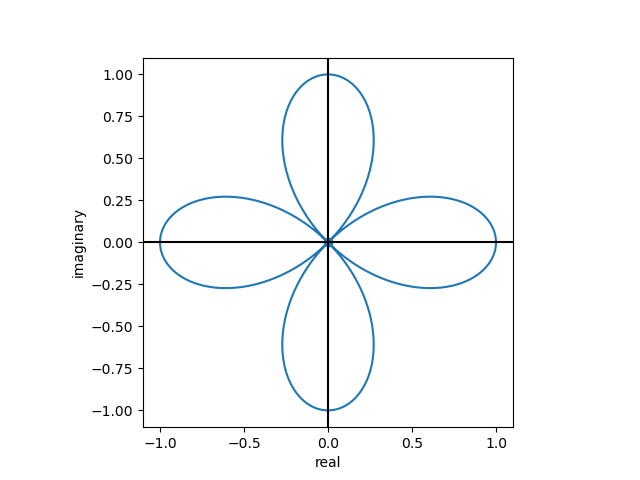
\includegraphics[width=0.4\textwidth]{cos_wrapped}}
    \end{figure}
    However, if we map the values to a circle with matching frequency $k$, we 
    observe something interesting - Figure~\ref{fig:cos_wrapped_2k}. All values
    have moved to one side, so now, if we sum all the values, we get a complex
    number. In the case of cosine, the result is real, which means that we 
    the function consists of a sinewave with $0$ phase change and amplitude of
    $1$ (the raw results from DFT have to be divided by $N$ to get representation
    below and by $2N$ to get the real amplitude).
    \begin{figure}[H]
        \caption{}
        \centering
        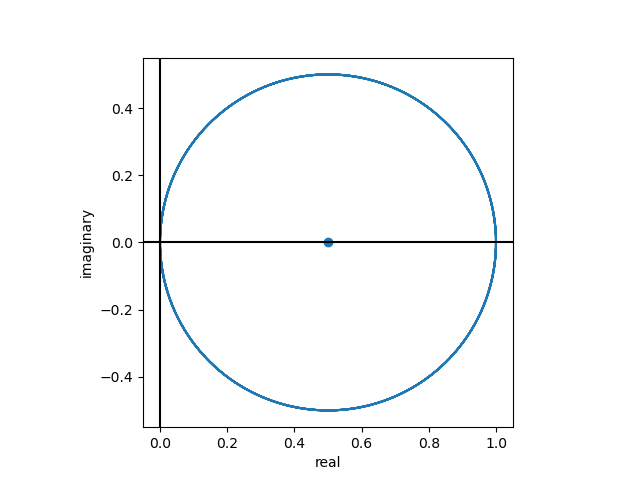
\includegraphics[width=0.4\linewidth]{cos_wrapped_2k}
        \label{fig:cos_wrapped_2k}
    \end{figure}
    If we wrap $sin(2t)$ the same way, we will see that we will have the phase
    change represented by the complex component - Figure~\ref{fig:sin_wrapped_2k}.
    This should make intuitive sense, because we saw that cosine function starts
    at completely horizontal position and the sine starts from completely vertical
    position. 
    \begin{figure}[H]
        \caption{}
        \centering
        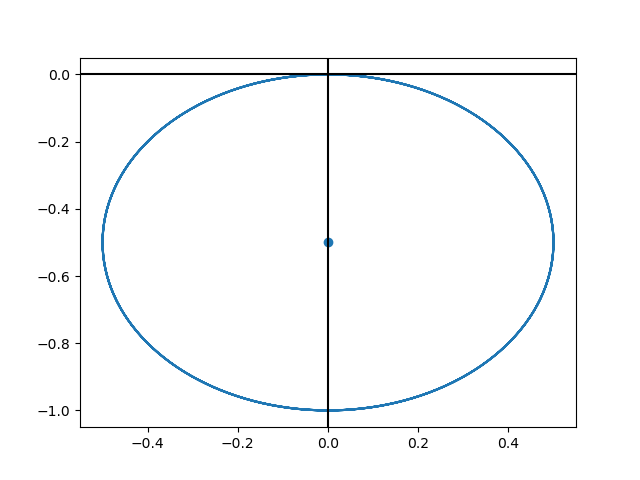
\includegraphics[width=0.4\linewidth]{sin_wrapped_2k}
        \label{fig:sin_wrapped_2k}
    \end{figure}
    We can already see that we will use DFT to set radii and initial positions
    of our ``circles'' that will spin at $k$ frequencies. Before that let us have
    one last bit of fun with DFT and decompose a function with more than one 
    component sine wave, say $f(t) = cos(10t) + cos(20t) + sin(25t)$, which looks
    like in Figure~\ref{fig:composed}. Now, all we have to do is apply Fourier
    transform.
    \begin{figure}[H]
        \caption{}
        \centering
        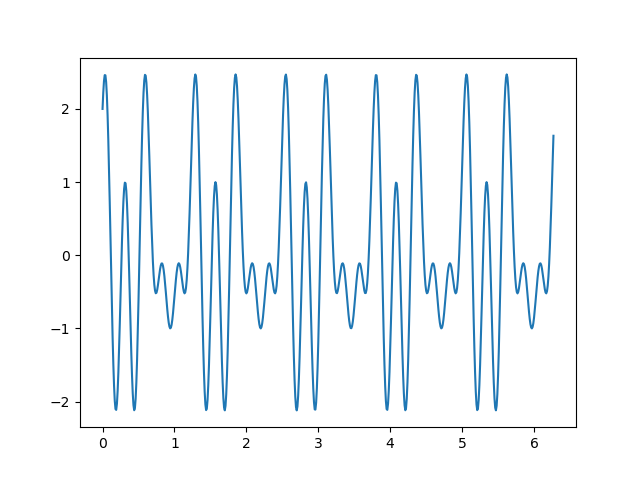
\includegraphics[width=0.4\linewidth]{composed}
        \label{fig:composed}
    \end{figure}
    Here are plots of our function mapped to the unit circle with following
    frequencies: $1, 10, 20, 25$, where the dot signifies the sum mapped with 
    $\frac{1}{N}$
    \begin{figure}[H]
    \caption{}
    \begin{tabular}{cc}
    \subfloat[k = 1]{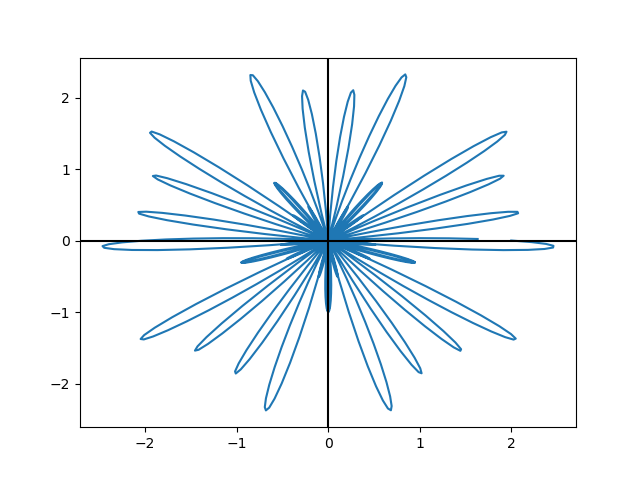
\includegraphics[width=0.4\linewidth]{composed_wrapped}} &
    \subfloat[k = 10]{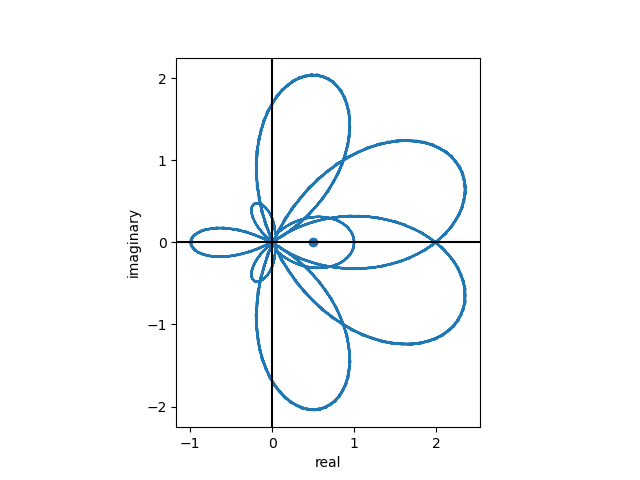
\includegraphics[width=0.4\linewidth]{decomposed_1}}\\
    \subfloat[k = 20]{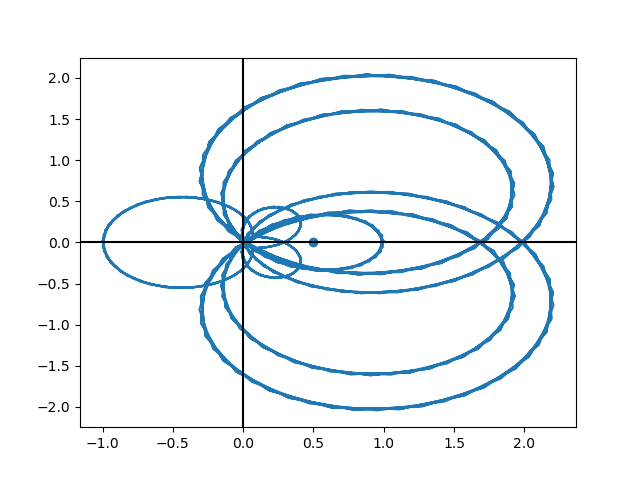
\includegraphics[width=0.4\linewidth]{decomposed_2}} &
    \subfloat[k = 25]{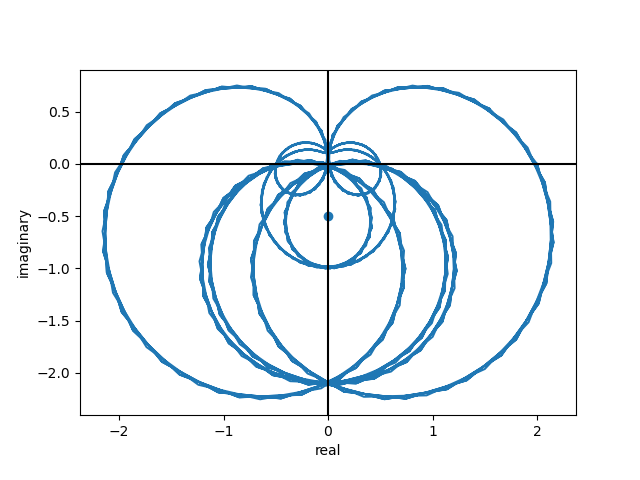
\includegraphics[width=0.4\linewidth]{decomposed_3}}
    \end{tabular}
    \label{step_fs_plots}
    \end{figure}
    
    See Appendix B for source code of script used to generate all plots above.

\subsubsection{Why naive implementation of DFT is inefficient}

    Now we can take a look at how DFT is implemented in C++.

    \begin{minted}{C++}

C_set *DFT(C_set input)
{
    C_set *out = new C_set;
    C temp, X_k;
    unsigned N = input.size();
    double a = (2 * M_PI) / N, x;

    for (unsigned k = 0; k < N; ++k)
    {
        for (unsigned n = 0; n < N; ++n)
        {
            x = a * n * k;
            temp.re = cos(x);
            temp.im = -sin(x);

            X_k += (temp * input[n]);
        }

        out->push_back(X_k);
        X_k = C(0,0);
    }

    return out;
}
    \end{minted}

    The function takes set of complex numbers which is our drawing and calculates
    coefficients for frequencies from $0$ to $N-1$. Of course this number could
    be arbitrarly high, but $N$ seems to do the trick. The algorithm is a direct
    implementation of the formula and the source of inefficiency is in the two
    nested for loops that go from $0$ to $N$. What this means is that the algorithm
    has the time complexity of $O(N^2)$, which means that supplied set of $N$ elements,
    the computer will always perform $N^2$ operations because the function does
    not contain any break statements which could add best and worst case scenario
    to the considerations. In real world, this algorithm is rarely used, as it has
    its much more efficient counterpart - 
    Fast Fourier Transform (FFT), which has the 
    complexity of $O(Nlog(N))$ which is significantly faster than $O(N^2)$, but 
    since the program is made as a bit of fun, we can live with poor efficiency.
    


\subsection{Fourier series and making drawings}

    At this point we have a set of complex numbers describing our sketch in terms
    of frequency and we have to come back to time domain. To do that we use inverse
    discrete Fourier transform (IDFT), which might as well be called discrete 
    Fourier series. Akin to approximating step function in section 2, we have 
    a bunch of weights on our hands and all we have to do is apply them to what
    we will now call our rotating circles - epicycles. DFT gives us two pieces
    of information about each frequency - how big is the epicycle and where is
    starts. The formula for IDFT is as follows~\eqref{eq:IDFT}
    \begin{equation}\label{eq:IDFT}
        x_n = \frac{1}{N}\sum_{n=0}^{N-1}X_k \cdot \left[cos\left(\frac{2\pi}{N}kn\right) +
        isin\left(\frac{2\pi}{N}kn\right)\right]
    \end{equation}
    Notice that what we are doing is applying Fourier transform to Fourier transform.
    The $\frac{1}{N}$ weight is the same weight we applied when depicting DFT.
    Now, having all tools needed, we can take a look at the code. Our goal is to
    control the number of terms. Provided that number, we can calculate the set 
    making up our drawing by adding $n$ for every angle from $0$ to $2\pi$. 
    Below is function called \textit{draw IDFT}, which does just that.
    \begin{minted}{C++}
void draw_IDFT(C_set &x_k, VertexArray &drawing, unsigned n)
{
    C temp, x_n;
    unsigned N = x_k.size();
    double step = (2 * M_PI) / N, theta;

    for (unsigned t = 0; t < N; ++t)
    {
        for (unsigned k = 0; k < n; ++k)
        {
            theta = step * t * k;     
            temp = C(cos(theta), sin(theta));

            x_n += (temp * x_k[k]) / N;
        }

        drawing[t] = Vector2f(x_n.re + 400, -x_n.im + 400);
        x_n = C(0,0);
    }
}
    \end{minted}
    If we go look at the code, it looks very similar to DFT implementation complete
    with that doubly nested loops. Starting from the top for loop, we have variable
    $t$, which is there to iterate over the full range, so in other terms - make 
    one full revolution at frequency $1$. The next loop is what allows us to observe
    the convergence to our input. Variable $k$, consistent with previous variable-
    naming is our frequency. Inside the loop, we are calculating the angle at which
    epicycle revolving at frequency $k$ is, after which we express it as a complex
    number in variable $temp$ to finally calculate its position using IDFT. We
    are adding the terms to $x_n$, since we want the outline rather than path of 
    each epicycle. Having calculated $x_n$, we add it to the buffer holding points
    making up our drawing. Rince and repeat.

\section{Drawings}

    This moment might be somewhat anticlimactic, since the program works best as
    a kind of animation, I will leave link to code repository complete with 
    instructions to compile the program. In this paper, however I will show off
    some simpler sketches that converge fast so that we can see it well without
    perusing a 100-page document containing every frame. 

\subsection{Triangle}

    \begin{figure}[H]
    \centering
    \caption{}
    \begin{tabular}{ccc}
    \subfloat[original input]{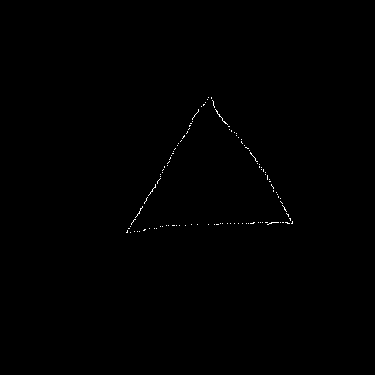
\includegraphics[width=0.3\linewidth]{fd_triangle_input}} &
    \subfloat[n = 2]{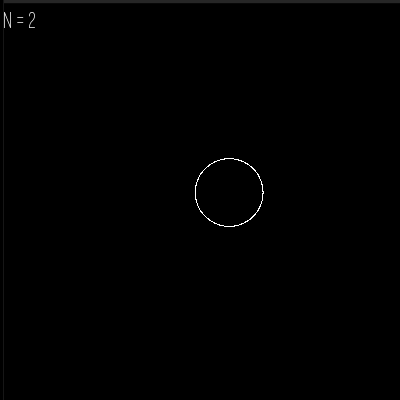
\includegraphics[width=0.3\linewidth]{fd_triangle_1}} &
    \subfloat[n = 15]{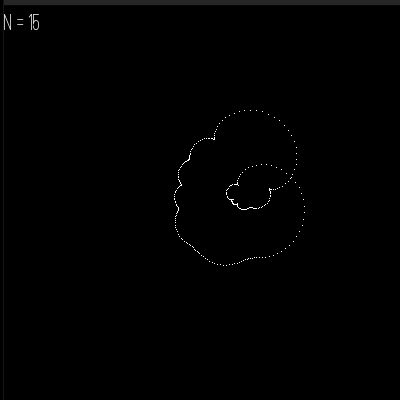
\includegraphics[width=0.3\linewidth]{fd_triangle_2}}\\
    \subfloat[n = 239]{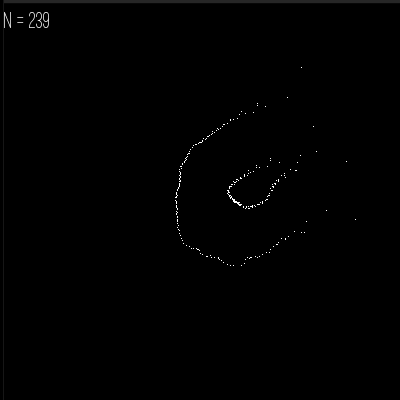
\includegraphics[width=0.3\linewidth]{fd_triangle_3}} &
    \subfloat[n = 314]{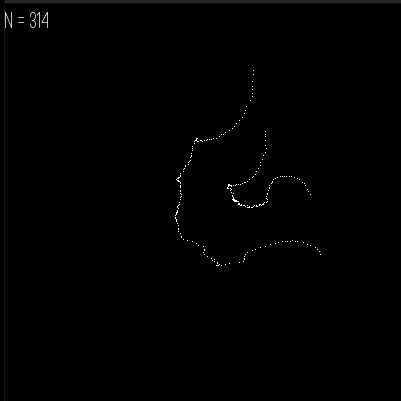
\includegraphics[width=0.3\linewidth]{fd_triangle_4}} &
    \subfloat[n = 322]{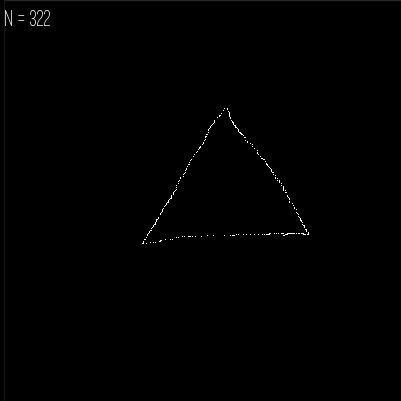
\includegraphics[width=0.3\linewidth]{fd_triangle_6}} 
    \end{tabular}
    \label{fig:triangles}
    \end{figure}
    
\subsection{Cube}

    \begin{figure}[H]
    \centering
    \caption{}
    \begin{tabular}{ccc}
    \subfloat[original input]{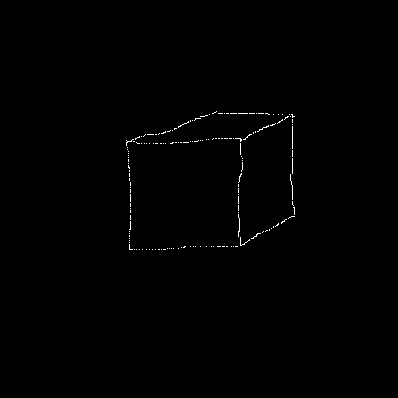
\includegraphics[width=0.3\linewidth]{fd_cube_input}} &
    \subfloat[n = 2]{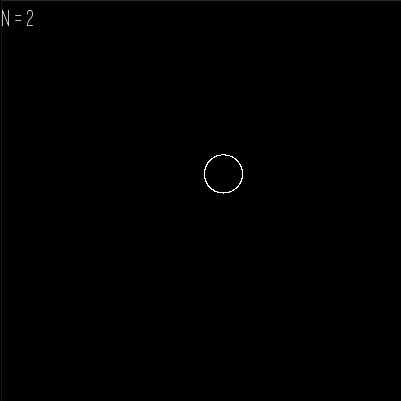
\includegraphics[width=0.3\linewidth]{fd_cube_1}} &
    \subfloat[n = 15]{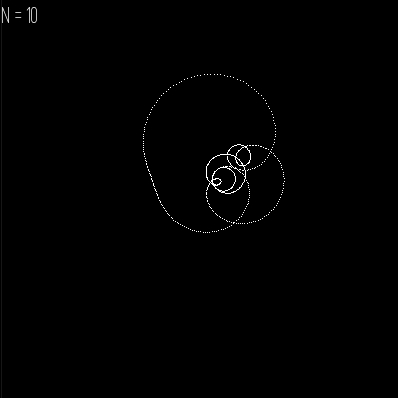
\includegraphics[width=0.3\linewidth]{fd_cube_2}}\\
    \subfloat[n = 239]{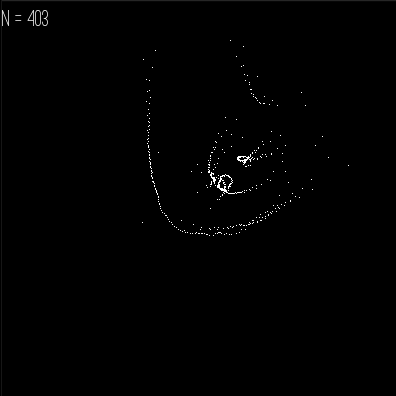
\includegraphics[width=0.3\linewidth]{fd_cube_3}} &
    \subfloat[n = 314]{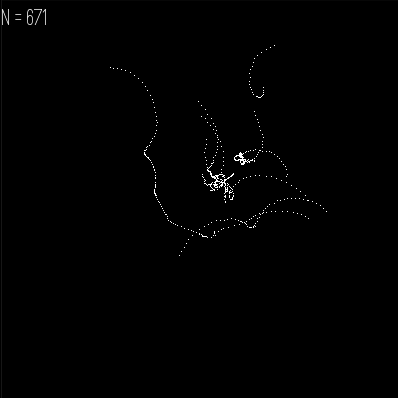
\includegraphics[width=0.3\linewidth]{fd_cube_4}} &
    \subfloat[n = 322]{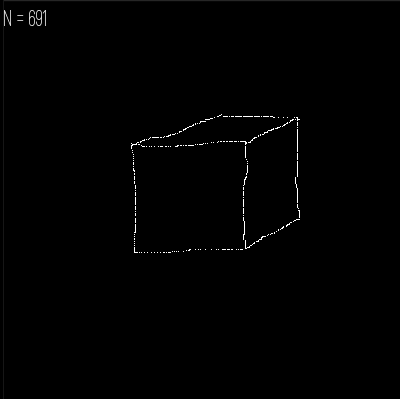
\includegraphics[width=0.3\linewidth]{fd_cube_6}} 
    \end{tabular}
    \label{fig:cubes}
    \end{figure}

\subsection{Pi}

    \begin{figure}[H]
    \centering
    \caption{}
    \begin{tabular}{ccc}
    \subfloat[original input]{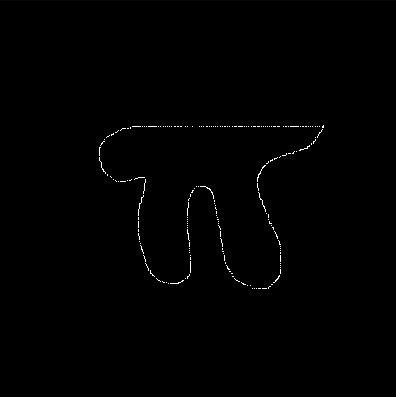
\includegraphics[width=0.3\linewidth]{fd_pi_input}} &
    \subfloat[n = 2]{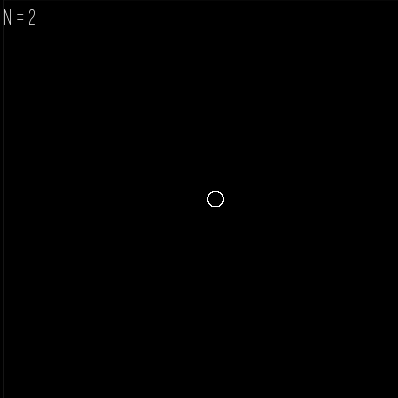
\includegraphics[width=0.3\linewidth]{fd_pi_1}} &
    \subfloat[n = 15]{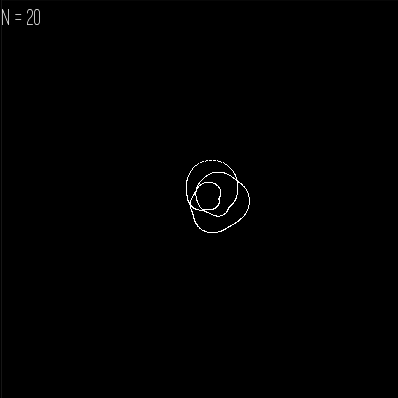
\includegraphics[width=0.3\linewidth]{fd_pi_2}}\\
    \subfloat[n = 239]{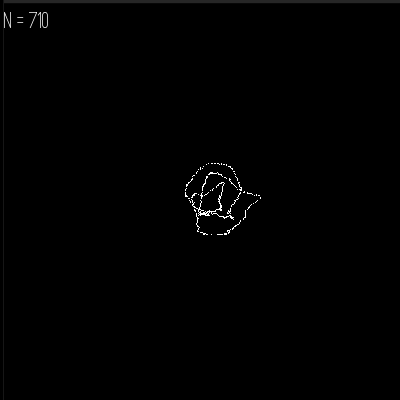
\includegraphics[width=0.3\linewidth]{fd_pi_3}} &
    \subfloat[n = 314]{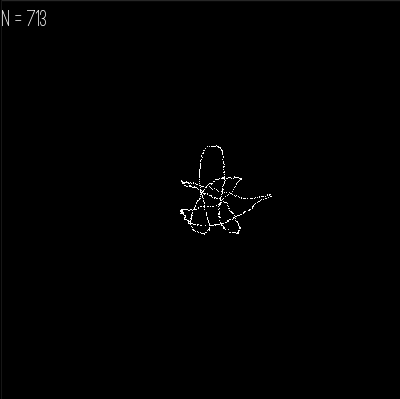
\includegraphics[width=0.3\linewidth]{fd_pi_4}} &
    \subfloat[n = 322]{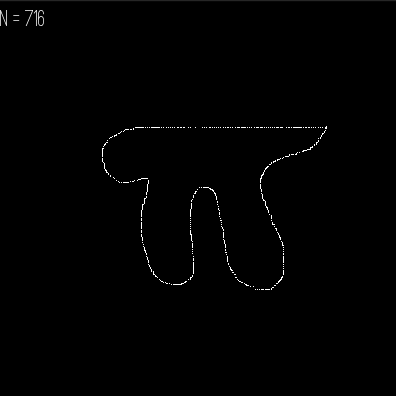
\includegraphics[width=0.3\linewidth]{fd_pi_6}} 
    \end{tabular}
    \label{fig:pis}
    \end{figure}

\section{Appendices}

\subsection*{Appendix A}


\end{document}
